\documentclass{article}

\title{TITLE}
\author{Adam Buskirk}

\usepackage{amssymb,amsmath,amsthm}
\usepackage{tikz}
\usepackage[margin=1in]{geometry}

\newtheorem{theorem}[subsection]{Theorem}
\newtheorem{conjecture}[subsection]{Conjecture}
\newtheorem{lemma}[subsection]{Lemma}
\theoremstyle{definition}
\newtheorem{definition}[subsection]{Definition}

\newcommand{\R}{\mathbb{R}}
\newcommand{\N}{\mathbb{N}}
\newcommand{\Q}{\mathbb{Q}}
\newcommand{\Z}{\mathbb{Z}}
\newcommand{\Co}{\mathbb{C}}
\newcommand{\p}[1]{\left(#1\right)}
\newcommand{\sq}[1]{\left[#1\right]}
\newcommand{\set}[1]{\left\{#1\right\}}
\newcommand{\abs}[1]{\left|#1\right|}
\newcommand{\norm}[1]{\left|\left|#1\right|\right|}
% \newcommand{\p}[1]{\left(#1\right)}

\begin{document}
\maketitle
\begin{figure}[h]
\centering
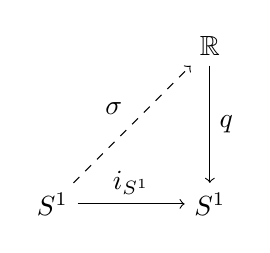
\begin{tikzpicture}[scale=2]
\node (A) at (0,0) {$S^1$};
\node (B) at (1,0) {$S^1$};
\node (C) at (1,1) {$\R$};
\draw[->] (A) to node[above] {$i_{S^1}$} (B) ;
\draw[->,style=dashed] (A) to node[above left] {$\sigma$} (C) ;
\draw[->] (C) to node[right] {$q$} (B) ;
\end{tikzpicture}
\end{figure}
Such a $\sigma$ lift cannot be found. Note that $i_{S^1} = q \circ \sigma$
implies that $\sigma$, $q|_{\operatorname{Im}(\sigma)}$ are injective. 
$\operatorname{Im}(\sigma)$ is a connected compact subset of $\R$, and thus
a closed interval $[a,b]$. If 

\end{document}
